% =====================================================================
%  Chapter 7 — Density, Rubble Pile\idx{Rubble pile} and Monolith
% =====================================================================

\chapter{Density, Rubble Pile and Monolith}
\label{ch:density}

The previous chapter ended with a measurement that removes the diameter
uncertainty. This chapter asks what remains, and the answer is the density:
the second factor of three in the energy relation, and the harder of the two
to obtain.

\section{Where the factor of three comes from}

A small body's bulk density is the product of its skeletal grain density and
its porosity, and its porosity is a statement about whether the body is a
coherent pile of fragments or a single bonded object. A rubble pile\idx{Rubble pile} of
fragments with the same grain density as a coherent body carries a void
fraction, and a typical void fraction of forty per cent reduces the bulk
density to three fifths of the solid value. That ratio, inverted, is the
factor of about three that separates the two populations.

The range is therefore not a measurement uncertainty in the ordinary sense.
It is a choice between two physical models of the object, and the object is
one or the other. The 2024~YR4 model set brackets it explicitly: 1,300
kilogrammes per cubic metre for a rubble pile\idx{Rubble pile} and 3,500 for a coherent body,
a ratio of 2.69, which propagates directly into the energy.

\section{How density is measured, and when}

There are four routes, and they are available at very different moments in
an object's life.

Radar polarimetry\idx{Polarimetry} measures the scattering signature of the regolith and can
distinguish a consolidated surface from a particulate one. It requires a
radar target, which in practice means proximity, and it is the most direct
surface-diagnostic of the four.

Thermal inertia measures how quickly the surface temperature responds to
insolation, and therefore how fine-grained and how loose the regolith is.
It is inferred from the shape of the thermal emission curve through a
rotation, and it constrains the regolith rather than the bulk body.

Flyby imaging measures the volume directly and the bulk density follows from
a separately determined mass. It is the most complete route and it is
available only to the handful of objects a spacecraft has visited.

The fourth route is the one this book is interested in, because it is the one
that scales: \emph{the close approach}. During an encounter inside the
gravitational sphere of influence of a massive body, the trajectory of the
object carries the imprint of that body's mass\idx{Mass}, and the imprint is
measurable.

\section{Why a close approach reveals the mass distribution}

The mechanism is subtle and it is worth stating carefully, because it is the
step that links the probability chain to the accounting chain.

An asteroid's mass\idx{Mass} and its internal mass\idx{Mass} distribution determine how it
responds to a gravitational perturbation. A spherical, rigid body and a
tumbling, elongated body with a concentrated mass distribution respond
differently to the same flyby: the same impulse along-track changes the
rotation rate of one and the rotation axis of the other, by different
amounts. The observable that changes is the spin state.

The 2022 study of Apophis's non-principal-axis rotation through its 2029
Earth encounter quantifies this. Working with refined orbit, spin-state and
inertia information from optical and radar observations, and propagating the
coupled orbital and rigid-body attitude dynamics through the encounter, it
finds that the gravitational changes to the tumbling periods and to the
rotational angular momentum direction are likely to be significant and
measurable. Apophis is likely to remain in a short-axis-mode tumbling state,
but its effective spin rate could halve or double, and its pole is likely to
shift by ten degrees or more and to move closer to the ecliptic plane. The
study is explicit that these changes are very sensitive to the close-approach
attitude and to the mass distribution --- and explicit about the
consequence: ground-based tracking of the spin state\idx{Spin state} through the encounter
will help refine the mass distribution.

That is the link. The spin state\idx{Spin state} is measurable from the ground with
photometry and a resolved shape. The mass distribution is not measurable from
the ground at all, except through the encounter. And the encounter is the one
occasion on which the mass distribution becomes observable at all.

\begin{seamnote}{This is why the shape and the density belong in one proposal}
A resolved shape measurement and a close-approach mass measurement are not
two independent capabilities that happen to be useful together. They are two
measurements of the same encounter: the shape supplies the volume, the
encounter supplies the mass, and the density is their quotient. An
architecture that can do the first and be present for the second closes the
entire energy chain, and an architecture that can do only the first closes
half of it.
\end{seamnote}

\section{What the density is worth at long horizons}

The last piece is the payoff, and it comes from the probability side of the
ledger. In the impact-probability study of Apophis's 2036 encounter, the
published sensitivity table varies one physical assumption at a time and
reports the resulting impact probability against the nominal case of
\(7.07\times 10^{-9}\).

\begin{table}[!htbp]
\centering
\small
\caption{The 2036 keyhole: the published sensitivity of the impact
probability to physical assumptions, against a nominal \(7.07\times10^{-9}\).}
\label{tab:bottke}
\begin{tabularx}{\textwidth}{@{}P{1.92in}P{1.27in}P{1.08in}@{}}
\toprule
\rowcolor{panel}
\textbf{Varied assumption} & \textbf{Impact probability} & \textbf{Factor} \\
\midrule
Nominal & \(7.07\times 10^{-9}\) & 1 \\
\rowcolor{panel}
Diameter 270 \(\pm\) 60 m & \(3.06\times 10^{-6}\) & 433 \\
Uniform \(\cos\gamma\) & \(2.67\times 10^{-9}\) & 0.38 \\
\rowcolor{panel}
Symmetric \(\cos\gamma\) & \(1.64\times 10^{-9}\) & 0.23 \\
Density variance, \(\sigma_\rho^{2} = 0.6\) & \(6.60\times 10^{-7}\) & 93 \\
\rowcolor{panel}
\(\mu_{d0} = 200\) & \(1.58\times 10^{-9}\) & 0.22 \\
\(\mu_{d0} = 400\) & \(1.59\times 10^{-8}\) & 2.25 \\
\bottomrule
\end{tabularx}
\end{table}

Two lines in \tabref{tab:bottke} carry the argument of this book. The
diameter assumption alone moves the impact probability by a factor of 433.
The density variance moves it by a factor of 93. Both are physical
assumptions, both are the kind of assumption a characterisation campaign is
designed to remove, and neither is touched by additional astrometry.

\begin{figure}[!htbp]
\centering
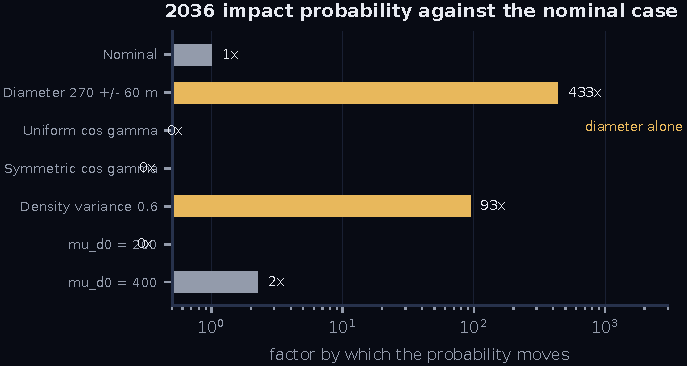
\includegraphics[width=\textwidth]{../figures/fig_keyhole.pdf}
\caption{The 2036 keyhole magnifies physical error. The diameter assumption
alone moves the impact probability by a factor of 433, and the density
variance by a factor of 93.}
\label{fig:keyhole}
\end{figure}

\figref{fig:keyhole} is the reason the book does not stop at shape. A
measurement that removes the diameter assumption removes the largest single
term in the table. A measurement that also removes the density assumption
removes the second largest. Both are attainable, both are attainable at the
same encounter, and neither is attainable by adding telescope time to an
existing programme.

\begin{keytakeaways}
\item The density range between a rubble pile and a coherent body is a factor
of about 2.7 in mass, and it is a choice between physical models rather than
a measurement noise.
\item A close approach reveals the mass distribution through its effect on
the spin state\idx{Spin state}, and the spin state is measurable from the ground.
\item The published 2029 Apophis study finds the spin rate could halve or
double and the pole could shift by ten degrees or more, and states that
tracking that change refines the mass distribution.
\item At the 2036 keyhole the density assumption is worth a factor of 93 in
the impact probability, and the diameter assumption a factor of 433.
\end{keytakeaways}
